% LNCS template: https://www.overleaf.com/latex/templates/springer-lecture-notes-in-computer-science
\documentclass[runningheads]{llncs}

\usepackage[a4paper, left=3cm, right=3cm, top=3.5cm, bottom=3.5cm]{geometry}

\usepackage{xurl}
\urlstyle{tt}
\usepackage{tabularx}
\usepackage{booktabs}
\usepackage[T1]{fontenc}
\usepackage{graphicx}
\usepackage{booktabs}
\usepackage{amsmath}
\usepackage{amssymb}
\usepackage{url}
\usepackage[hidelinks]{hyperref}
\usepackage{xcolor}
\usepackage{listings}
\usepackage{multirow}
\usepackage{tikz}
\usetikzlibrary{arrows.meta,positioning}

\lstset{
  basicstyle=\ttfamily\small,
  breaklines=true,
  frame=single,
  backgroundcolor=\color{gray!10},
}

\begin{document}

\title{Explainable GNN on the AIFB Knowledge Graph:\\
Global Explanations via Description Logic Concept Learning}

% Add this command to fix the running header error:
\titlerunning{Global Explanations via DL Concept Learning on AIFB GNN}

\author{Mukund Chavda, Bofeng Duan, Marta Ravazzoni}

\institute{University of Paderborn, Germany\\
\{mchavda, bofeng, rmarta\}@mail.uni-paderborn.de}

\maketitle

%---------------------------------------------------------------------
\begin{abstract}
We present an explainable AI pipeline for node classification on the AIFB academic knowledge graph.
The system trains a Relational Graph Convolutional Network (R-GCN) to predict the research group
affiliation of 176 researchers and then derives global, symbolic explanations from the model's
predicted classes using description-logic concept learning (Strategy~3).
The final AIFB configuration uses RDF-neighbourhood feature vectors that encode node types,
literal attributes, and typed outgoing relations, achieving \textbf{94.4\,\%} test accuracy.
The explanation stage translates the trained classifier's output into class-level hypotheses such as
publication-cardinality and role-restriction concepts, making the learned graph patterns inspectable.
\end{abstract}

%---------------------------------------------------------------------

\setcounter{tocdepth}{2}
\tableofcontents
\clearpage

\section{Introduction}

Knowledge graphs (KGs) encode relational information as RDF triples $(s, p, o)$ and form the backbone
of applications from biomedical databases to enterprise search.
Graph Neural Networks (GNNs) are a natural fit for this setting because they can aggregate information
over typed graph neighbourhoods.  However, a predicted label alone does not tell us which graph patterns
the model relied on.  This project therefore combines prediction with a symbolic post-hoc explanation step.

\textbf{Task definition.}
Given the AIFB KG, which describes researchers at the University of Karlsruhe, we predict the
\emph{research group} of each person (a 4-class classification problem).
Label-leaking predicates (\texttt{affiliation}, \texttt{employs}) are excluded so the model must learn
structural and semantic patterns rather than reading the answer directly.

\textbf{Our approach.}
We follow \emph{Strategy~3} from the course mini-project guidance~\cite{xai26miniproject}: train an R-GCN on the KG, then use the model's predictions
as positive/negative examples for a concept learner (CELOE via Ontolearn~\cite{ontolearn2023}).
The concept learner outputs description-logic formulae that compactly characterise each predicted class.

\textbf{Contributions.}
\begin{itemize}
    \item We implement an AIFB-focused pipeline: RDF parsing $\to$ feature extraction $\to$ R-GCN training $\to$ DL explanation.
    \item We replace node-ID embeddings with \emph{rdf\_neighborhood} features, i.e. sparse multi-hot vectors that encode RDF type, literal attributes, and typed neighbourhood context.
    \item We evaluate the best AIFB experiment and analyse how the generated description-logic hypotheses reflect the classifier's learned decision patterns.
\end{itemize}

\paragraph{Code availability.}
The final implementation, AIFB data files, experiment configurations, and reproduction instructions are available on GitHub at
\url{https://github.com/the-m-chavda/xai-mini-project}.

%---------------------------------------------------------------------
\section{Data Analysis}

\subsection{Dataset Overview}

The AIFB dataset~\cite{bloehdorn2007} is an academic knowledge graph describing the AIFB research institute
at the University of Karlsruhe.
It contains persons, publications, projects, and research topics connected by 44 relation types.
The classification target is the \emph{research group affiliation} of 176 selected researchers.

\begin{table}[ht]
\centering
\caption{AIFB dataset statistics.}
\label{tab:dataset}
\begin{tabular}{lr}
\toprule
\textbf{Statistic} & \textbf{Value} \\
\midrule
Total RDF triples       & 29,226 \\
Resource triples        & 20,521 \\
Literal triples         & 8,705  \\
Model nodes             & 2,835  \\
Model edges (with inv.) & 40,676 \\
Relation types          & 44     \\
Target entities         & 176    \\
\quad Training set      & 140    \\
\quad Test set          & 36     \\
Classes (research groups) & 4    \\
\bottomrule
\end{tabular}
\end{table}

Table~\ref{tab:dataset} was generated by parsing the RDF file and the official train/test label splits.
The most important observation is that the supervised task is small (176 labelled persons), while the
message-passing graph is much larger and contains thousands of publication and project nodes that can
provide context.

\subsection{Class Distribution}

The four research groups are highly imbalanced (Table~\ref{tab:labels}),
with \emph{Complexity Management} containing only 15 members---roughly 8.5\,\% of the dataset.
This imbalance poses a challenge both for the classifier and for the concept learner,
which receives fewer positive examples for the minority class.

\begin{table}[ht]
\centering
\caption{Label distribution in the AIFB dataset.}
\label{tab:labels}
\begin{tabular}{lrr}
\toprule
\textbf{Research Group} & \textbf{Members} & \textbf{Share} \\
\midrule
Business Information \& Communication Systems & 73 & 41.5\,\% \\
Knowledge Management                          & 60 & 34.1\,\% \\
Efficient Algorithms                          & 28 & 15.9\,\% \\
Complexity Management                         & 15 &  8.5\,\% \\
\midrule
\textbf{Total}                                & \textbf{176} & 100\,\% \\
\bottomrule
\end{tabular}
\end{table}

\subsection{Graph Structure}

The most frequent node types are \emph{Publication} (1,222), \emph{Person} (1,045),
\emph{InProceedings} (687), \emph{TechnicalReport} (169), and \emph{Article} (161).
The excluded predicates \path{swrc:affiliation} and \path{swrc:employs}
directly encode group membership and must be removed to prevent label leakage.
After exclusion, the model must rely on co-authorship networks, publication types,
and project memberships to infer group affiliation.

%---------------------------------------------------------------------
\section{Model Training and Evaluation}

\subsection{From RDF Triples to a Supervised Graph Problem}

The modelling problem is not a standard tabular classification task.  Each example is a person in an
RDF knowledge graph, and most useful information is relational: a researcher is connected to publications,
projects, research topics, and other academic entities through typed predicates.  A model that only sees
one row per person would discard precisely the structure that makes the AIFB dataset interesting.
We therefore first turn the RDF graph into a multi-relational directed graph and then train a graph neural
network over this graph.

Let the RDF graph be a set of triples $(s,p,o)$, where $s$ and $o$ are resources or literals and $p$ is an
RDF predicate.  We construct a graph $G=(V,E,\mathcal{R})$ as follows.  URI resources and blank nodes become
graph nodes.  For each non-literal triple whose predicate is not label-leaking, we add a typed edge
$(s,p,o)$.  We also add an inverse edge $(o,p^{-1},s)$, because useful information should flow both from
persons to publications and from publications back to persons.  Direct group-membership predicates
\texttt{swrc:affiliation} and \texttt{swrc:employs} are removed before graph construction.  This is essential:
otherwise the classifier and the explainer could recover the answer directly from the graph.

The resulting training graph contains 2,835 nodes, 40,676 directed edges after adding inverses, and 44
relation types.  The labelled subset consists of 176 persons, split into 140 training examples and 36 test
examples.  The model is trained only on labelled persons, but message passing uses the full leakage-filtered
graph, so unlabeled publications, projects, and topics can still provide context.

\subsection{Why a Relational GCN?}

A vanilla GCN assumes that all neighbours are connected by the same kind of edge.  This assumption is too
coarse for RDF data and typed knowledge graphs~\cite{xai26xgnn}: a \texttt{publication} edge, an \texttt{author} edge, and a \texttt{hasProject} edge
carry different meanings.  Treating them as identical would blur together heterogeneous evidence.  An
R-GCN~\cite{schlichtkrull2018} addresses this by learning a separate transformation for each relation type while still sharing the
same message-passing framework across the whole graph.

For node $v$ at layer $l$, our R-GCN layer computes
\[
h_v^{(l+1)} =
\mathrm{Dropout}\!\left(
\mathrm{ReLU}\!\left(
W_{\mathrm{self}}^{(l)} h_v^{(l)}
  + \sum_{r \in \mathcal{R}} \sum_{u \in \mathcal{N}_r(v)}
    \frac{1}{|\mathcal{N}_r(v)|} W_r^{(l)} h_u^{(l)}
  + b^{(l)}
\right)\right),
\]
where $\mathcal{N}_r(v)$ is the set of incoming neighbours of $v$ under relation $r$.
The relation-specific matrix $W_r^{(l)}$ tells the layer how to transform messages arriving through
relation $r$, while $W_{\mathrm{self}}^{(l)}$ preserves the node's own representation.  Degree
normalisation prevents high-degree nodes from dominating the aggregation simply because they have many
neighbours.

The final architecture is deliberately small but expressive enough for AIFB:
\[
X \xrightarrow[]{\mathrm{Linear}(4017,64)}
H^{(0)} \xrightarrow[]{\mathrm{RGCN}(64,128)}
H^{(1)} \xrightarrow[]{\mathrm{RGCN}(128,128)+\mathrm{residual}}
H^{(2)} \xrightarrow[]{\mathrm{Linear}(128,4)}
\hat{Y}.
\]
The first R-GCN layer expands the projected input features from 64 to 128 dimensions.  The second layer
keeps the same hidden size, so a residual connection can be added around it.  Layer normalisation is applied
after each R-GCN layer.  In practice, the residual connection and normalisation make the two-layer model
less brittle: the second layer can refine the first layer's representation without destroying it.

\subsection{Node Representation: From Memorising IDs to Semantic Features}

\textbf{RDF-neighbourhood features.}
The final configuration represents each node with an explicit RDF feature vector rather than an arbitrary
node identity.  For each node
$v$, we build a sparse multi-hot vector $x_v \in \{0,1\}^{4017}$ (Table~\ref{tab:feature-families}). A shared input projection maps this
vector into the neural embedding space:
\[
h_v^{(0)} = W_{\mathrm{in}}x_v.
\]
The important difference is that $x_v$ is not an arbitrary node identity.  It records reusable graph
properties such as the node's RDF types, literal attributes, and the types of resources reached through
outgoing predicates.  Thus, if two researchers are both connected to projects, publications, or typed
academic entities in similar ways, the model can begin from partially shared evidence before any message
passing occurs.

\begin{table}[ht]
\centering
\small
\caption{Feature families in the AIFB RDF-neighbourhood representation.}
\label{tab:feature-families}
\begin{tabular}{@{}p{3.2cm}rp{6.5cm}@{}}
\toprule
\textbf{Feature family} & \textbf{Count} & \textbf{Example / purpose} \\
\midrule
RDF type & 27 & \texttt{type::Person}; captures ontology class membership. \\
Typed neighbourhood & 64 & \texttt{exists::publication::TechnicalReport}; captures typed outgoing context. \\
Literal predicate & 23 & \texttt{literal\_predicate::homepage}; records available literal attributes. \\
Literal datatype & 1 & \texttt{literal\_datatype::xsd:string}; records typed literal metadata. \\
Short literal value & 3,901 & short lexical attributes of publications/persons. \\
Fallback kind & 1 & marker for nodes without extracted RDF features. \\
\midrule
\textbf{Total} & \textbf{4,017} & sparse binary input vector \\
\bottomrule
\end{tabular}
\end{table}

Listing~\ref{lst:features} summarises the feature extraction procedure.  Literal nodes are not inserted as
message-passing nodes in the graph, but their predicates, datatypes, and short values are attached as
features to the subject resource.  For resource-valued objects, we first collect their RDF types and then
add typed-existence features to the subject.

\begin{lstlisting}[caption={RDF-neighbourhood feature extraction.},label={lst:features}]
Input: RDF graph G, excluded predicates E
Output: sparse feature list F[v] for each graph node v

object_types = {}
for (s, p, o) in sorted(G):
    if p == rdf:type:
        object_types[s].add(o)

for (s, p, o) in sorted(G):
    if p in E:
        continue
    if p == rdf:type:
        F[s].add("type::" + o)
    else if o is a literal:
        F[s].add("literal_predicate::" + p)
        F[s].add("literal_datatype::" + datatype(o))
        if len(value(o)) <= 64:
            F[s].add("literal_value::" + value(o))
    else if o is a resource:
        for t in object_types.get(o, {"Thing"}):
            F[s].add("exists::" + p + "::" + t)

for node v with no features:
    F[v].add("kind::resource_without_type")
\end{lstlisting}

This representation does not make the task inductive in the strict sense, because all test nodes are still
part of the transductive AIFB graph.  However, it substantially reduces the need to memorise arbitrary
node positions.  The model can learn weights for meaningful RDF patterns, and those weights are reused
wherever the same patterns appear.

\subsection{Training Procedure}

We train with cross-entropy loss on the labelled training persons.  To avoid selecting a checkpoint by
test performance, 15\,\% of the training labels are held out as a stratified validation split.  The
optimiser is Adam with learning rate 0.005 and weight decay 0.001.  The best checkpoint is selected by
validation macro-F1, which is more appropriate than raw accuracy for an imbalanced four-class dataset.
Listing~\ref{lst:training} gives the resulting training loop.

\begin{lstlisting}[caption={Training and checkpoint selection.},label={lst:training}]
Input: labelled train nodes T, test nodes S, graph G
Split T into fit set T_fit and validation set T_val
Build RDF-neighborhood matrix X
Initialise R-GCN parameters theta

best_state = None
best_val_f1 = -inf
patience_counter = 0

for epoch in 1..250:
    logits = RGCN_theta(G, X)
    loss = CrossEntropy(logits[T_fit], labels[T_fit])
    update theta with Adam

    val_f1 = MacroF1(argmax(logits[T_val]), labels[T_val])
    if val_f1 > best_val_f1:
        best_val_f1 = val_f1
        best_state = copy(theta)
        patience_counter = 0
    else:
        patience_counter += 1

    if patience_counter >= 30:
        break

Restore best_state
Report final train and test metrics
\end{lstlisting}

\begin{table}[ht]
\centering
\caption{R-GCN hyperparameters for the best AIFB experiment.}
\label{tab:hyperparams}
\begin{tabular}{ll}
\toprule
\textbf{Hyperparameter} & \textbf{Value} \\
\midrule
Initial features     & rdf\_neighborhood (4,017-dim) \\
Input projection     & Linear(4017, 64) \\
Hidden dim           & 128 \\
Number of R-GCN layers & 2 \\
Dropout              & 0.5 \\
Residual connections & yes, when dimensions match \\
Layer normalisation  & yes \\
Optimiser            & Adam \\
Learning rate        & 0.005 \\
Weight decay         & 0.001 \\
Validation fraction  & 15\,\% \\
Early stopping       & patience 30 \\
Max epochs           & 250 \\
\bottomrule
\end{tabular}
\end{table}

Table~\ref{tab:hyperparams} mirrors the final configuration file \texttt{configs/aifb.yaml}.  The validation
split and early stopping are included to avoid selecting a model by looking at the test set.

\subsection{Results and Error Pattern}

\begin{table}[ht]
\centering
\caption{Classification performance on AIFB.}
\label{tab:results}
\begin{tabular}{lcccc}
\toprule
\textbf{Features} & \textbf{Train Acc} & \textbf{Test Acc} & \textbf{Train F1} & \textbf{Test F1} \\
\midrule
rdf\_neighborhood model  & \textbf{98.6\,\%} & \textbf{94.4\,\%} & \textbf{0.984} & \textbf{0.912} \\
\bottomrule
\end{tabular}
\end{table}

The RDF-neighbourhood model reaches 94.4\,\% test accuracy and 0.912 test macro-F1, with a final
train--test accuracy gap of 4.2 percentage points.  The best validation macro-F1 is reached at epoch 25;
training stops at epoch 46 after 30 epochs without validation improvement, and the best checkpoint is
restored.  The final test result is 34/36 correct predictions.

\begin{table}[ht]
\centering
\caption{Test-set confusion matrix for the best AIFB model.}
\label{tab:confusion}
\begin{tabular}{lrrrr}
\toprule
\textbf{True class} & \textbf{BI} & \textbf{CM} & \textbf{EA} & \textbf{KM} \\
\midrule
Business Information (BI) & 15 & 0 & 0 & 0 \\
Complexity Management (CM) & 1 & 2 & 0 & 0 \\
Efficient Algorithms (EA) & 1 & 0 & 5 & 0 \\
Knowledge Management (KM) & 0 & 0 & 0 & 12 \\
\bottomrule
\end{tabular}
\end{table}

The confusion matrix shows that Knowledge Management and Business Information are classified perfectly
on the test split.  The two mistakes are both minority-class examples predicted as Business Information:
one Complexity Management person and one Efficient Algorithms person.  This is consistent with the class
distribution: Business Information is the largest class, and minority groups have fewer labelled examples
from which to learn class-specific patterns.

%---------------------------------------------------------------------
\section{Model Explanation}

\subsection{Explanation Strategy}

The classifier gives one label per person, but the project goal is not only to obtain a good accuracy
score.  We also want a compact description of the patterns that the trained model associates with each
research group.  We therefore use the Strategy~3 setting: after the R-GCN has been trained, its predictions
are converted into learning problems for a symbolic concept learner.

For each predicted class $c$, we define
\[
P_c = \{v \mid \hat{y}_v = c\}, \qquad
N_c = \{v \mid \hat{y}_v \neq c\}.
\]
Here, $P_c$ contains the persons that the R-GCN predicts as class $c$, and $N_c$ contains the remaining
labelled persons.  This means the explanations describe the model's behaviour, not the original labels
directly.  Positive examples are capped at 40 and negative examples at 80 after deterministic shuffling.
The ontology used for concept learning is the same leakage-filtered graph used for training, so
\texttt{swrc:affiliation} and \texttt{swrc:employs} are not available to the explainer.

\begin{table}[ht]
\centering
\caption{Learning-problem sizes constructed from R-GCN predictions.}
\label{tab:learning-problems}
\small
\begin{tabularx}{\textwidth}{Xrrr}
\toprule
\textbf{Predicted class} & 
\textbf{Predicted persons} & 
\textbf{Positives used} & 
\textbf{Negatives used} \\
\midrule
Business Information \& Communication Systems & 75 & 40 & 80 \\
Efficient Algorithms                          & 27 & 27 & 80 \\
Knowledge Management                          & 60 & 40 & 80 \\
Complexity Management                         & 14 & 14 & 80 \\
\bottomrule
\end{tabularx}
\end{table}

Table~\ref{tab:learning-problems} was created from the saved prediction file
\path{artifacts/aifb/predictions.csv}.
It shows that the explanation tasks inherit the class imbalance
of the original problem: the smallest predicted class, Complexity Management, has only 14 positive
examples.  This matters when interpreting the concepts, since small positive sets make precise global
rules harder to find.

\subsection{Explanation Pipeline}

Figure~\ref{fig:pipeline} summarizes the complete pipeline.  The figure was drawn from the actual
implementation stages: data preparation, R-GCN prediction model, and explanation model.  The main point is
that the explanation model does not replace the R-GCN.  It is a second stage that receives the trained
model's predictions and turns them into symbolic learning problems.

\begin{figure}[ht]
\centering
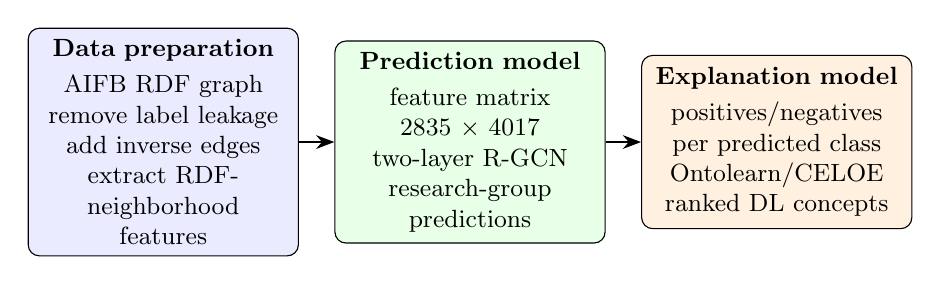
\begin{tikzpicture}[
    >=Stealth,
    node distance=0.45cm,
    stage/.style={draw, rounded corners, align=center, font=\small, text width=3.15cm, minimum height=2.2cm, inner sep=4pt}
]
\node[stage, fill=blue!8] (data) {
    \textbf{Data preparation}\\[2pt]
    AIFB RDF graph\\
    remove label leakage\\
    add inverse edges\\
    extract RDF-neighborhood features
};
\node[stage, fill=green!9, right=of data] (model) {
    \textbf{Prediction model}\\[2pt]
    feature matrix\\
    $2835 \times 4017$\\
    two-layer R-GCN\\
    research-group predictions
};
\node[stage, fill=orange!12, right=of model] (expl) {
    \textbf{Explanation model}\\[2pt]
    positives/negatives\\
    per predicted class\\
    Ontolearn/CELOE\\
    ranked DL concepts
};
\draw[->, thick] (data) -- (model);
\draw[->, thick] (model) -- (expl);
\end{tikzpicture}
\caption{End-to-end explainable AI pipeline for the AIFB experiment.}
\label{fig:pipeline}
\end{figure}

\subsection{Top Concept Hypotheses}

Ontolearn/CELOE returns ranked OWL class expressions for each predicted research group, together with a
quality (F1) score and, once intersected with the predicted positive/negative sets, precision and recall.
Table~\ref{tab:explanations-full} therefore reports the top three concepts per class with their fidelity
scores and a short reading of each expression.

\begin{table}[ht]
\centering
\scriptsize
\setlength{\tabcolsep}{3pt}
\caption{Top-3 Ontolearn/CELOE hypotheses for the best AIFB run, with fidelity to the R-GCN's predictions.}
\label{tab:explanations-full}
\begin{tabular}{@{}p{2.05cm}cp{3.05cm}p{1.55cm}p{3.4cm}@{}}
\toprule
\textbf{Class} & \textbf{Rank} & \textbf{DL concept} & \textbf{F1 / P / R} & \textbf{Plain reading} \\
\midrule
Business Information
  & 1 & $\forall\,\textit{member}^{-}.(\neg\textit{Project})$
  & 0.646 / 0.554 / 0.775
  & Incoming \textit{member} context is not project-like. \\
Business Information
  & 2 & $\forall\,\textit{publication}.(\neg\textit{InProceedings})$
  & 0.633 / 0.641 / 0.625
  & Publication neighbours are constrained away from \textit{InProceedings}. \\
Business Information
  & 3 & $\leq 0\,\textit{publication}.(\neg\textit{InProceedings})$
  & 0.633 / 0.641 / 0.625
  & Cardinality variant of the publication restriction. \\
\midrule
Efficient Algorithms
  & 1 & $\leq 6\,\textit{publication}.(\neg\textit{InProceedings})$
  & 0.436 / 0.289 / 0.889
  & At most six publication neighbours outside \textit{InProceedings}. \\
Efficient Algorithms
  & 2 & $\forall\,\textit{publication}.(\neg\textit{Misc})$
  & 0.435 / 0.284 / 0.926
  & Publication neighbours are not miscellaneous publications. \\
Efficient Algorithms
  & 3 & $\leq 0\,\textit{publication}.(\neg\textit{Misc})$
  & 0.435 / 0.284 / 0.926
  & Cardinality version of the non-\textit{Misc} restriction. \\
\midrule
Knowledge Management
  & 1 & $\neg\textit{Lecturer}$
  & 0.510 / 0.342 / 1.000
  & Predicted members are generally not typed as lecturers. \\
Knowledge Management
  & 2 & $\top$
  & 0.500 / 0.333 / 1.000
  & Very broad concept, indicating weak separability by a short rule. \\
Knowledge Management
  & 3 & $\neg\textit{Workshop}$
  & 0.500 / 0.333 / 1.000
  & Negative type restriction rather than a specific positive marker. \\
\midrule
Complexity Management
  & 1 & $\leq 5\,\textit{publication}.(\neg\textit{InProceedings})$
  & 0.321 / 0.194 / 0.929
  & Publication profile similar to Efficient Algorithms but stricter. \\
Complexity Management
  & 2 & $\leq 4\,\textit{publication}.(\neg\textit{InProceedings})$
  & 0.316 / 0.194 / 0.857
  & Even stricter non-\textit{InProceedings} cardinality bound. \\
Complexity Management
  & 3 & $\leq 1\,\textit{publication}.(\neg\textit{TechnicalReport})$
  & 0.311 / 0.184 / 1.000
  & Restriction involving non-technical-report publications. \\
\bottomrule
\end{tabular}
\end{table}

The table suggests that publication structure is one of the main sources of signal in the trained model.
This is consistent with the data analysis: \texttt{swrc:publication} and \texttt{swrc:author} are among the
most frequent predicates, while direct affiliation links have been removed.  Some concepts are intuitive
publication-profile descriptions, while others are broad negative restrictions.  We therefore treat them as
useful summaries of model behaviour, not as complete semantic definitions of the research groups.

\subsection{Example Explanation}

Figure~\ref{fig:example-explanation} gives a concrete example of how a learned concept can be read in graph
terms.  The example is based on the highest-scoring quantitative feature explanation for Knowledge
Management in Table~\ref{tab:explanation-eval}: $\exists\,\textit{publication}.\textit{TechnicalReport}$.
All node and edge labels in the figure are human-readable.  The explanation says that a person is covered
by the concept if the graph contains a publication edge from that person to a resource whose type is
\textit{TechnicalReport}.

\begin{figure}[ht]
\centering
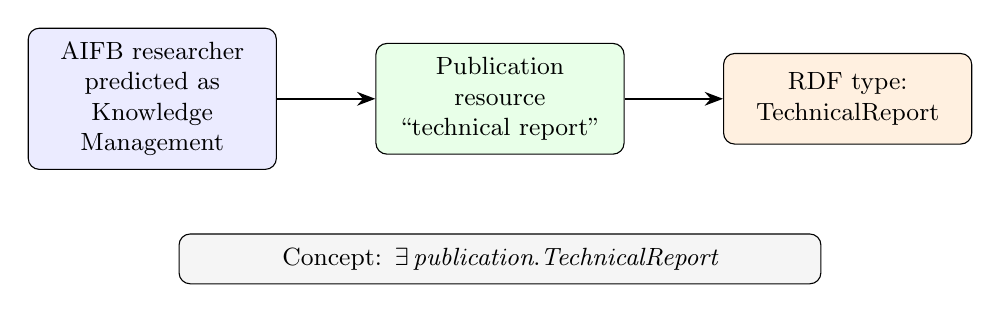
\begin{tikzpicture}[
    >=Stealth,
    node distance=1.15cm and 1.25cm,
    box/.style={
        draw,
        rounded corners,
        align=center,
        font=\small,
        text width=2.8cm,
        minimum height=1.15cm,
        inner sep=5pt
    },
    edge/.style={->, thick},
    edgelabel/.style={
        font=\scriptsize,
        fill=white,
        inner sep=1.5pt,
        midway,
        above
    }
]
\node[box, fill=blue!8] (person)
  {AIFB researcher\\predicted as\\Knowledge Management};

\node[box, fill=green!9, right=of person] (pub)
  {Publication resource\\``technical report''};

\node[box, fill=orange!12, right=of pub] (type)
  {RDF type:\\TechnicalReport};

\draw[edge] (person) -- node[edgelabel] { } (pub);
\draw[edge] (pub) -- node[edgelabel] { } (type);

\node[
    draw,
    rounded corners,
    fill=gray!8,
    align=center,
    font=\small,
    text width=7.8cm,
    below=1.0cm of pub,
    inner sep=5pt
] (concept)
  {Concept: $\exists\,\textit{publication}.\textit{TechnicalReport}$};

\end{tikzpicture}
\caption{Example explanation with human-readable node and edge labels.}
\label{fig:example-explanation}
\end{figure}

\section{Explanation Evaluation}

As a complementary, simpler baseline to CELOE's search over compound DL concepts, we also evaluate a set of
single-feature explanations using the same prediction-defined positive and negative examples.  For each
class, every candidate RDF-neighbourhood feature is treated as a simple concept.  We then compute precision,
recall, and F1 by checking how many positives and negatives are covered:
\[
\text{precision}=\frac{|\text{covered positives}|}{|\text{covered positives}|+|\text{covered negatives}|},
\quad
\text{recall}=\frac{|\text{covered positives}|}{|\text{all positives}|}.
\]
This is an automatic fidelity-style evaluation: it measures how well a readable concept approximates the
R-GCN's predicted class membership.

\begin{table}[ht]
\centering
\caption{Quantitative evaluation of the best feature-level explanations.}
\label{tab:explanation-eval}
\begin{tabular}{p{3.1cm}p{4.2cm}ccc}
\toprule
\textbf{Class} & \textbf{Best evaluated concept} & \textbf{Prec.} & \textbf{Rec.} & \textbf{F1} \\
\midrule
Business Information
  & \textsc{HasLiteral}(\textit{fax})
  & 0.333 & 1.000 & 0.500 \\
Efficient Algorithms
  & $\exists\,\textit{worksAtProject}.\textit{Project}$
  & 0.391 & 0.667 & 0.493 \\
Knowledge Management
  & $\exists\,\textit{publication}.\textit{TechnicalReport}$
  & 0.675 & 0.675 & \textbf{0.675} \\
Complexity Management
  & $\exists\,\textit{member}^{-}.\textit{ResearchGroup}$
  & 0.316 & 0.857 & 0.462 \\
\bottomrule
\end{tabular}
\end{table}

Table~\ref{tab:explanation-eval} was created from the same learning problems as
Table~\ref{tab:learning-problems}.  Knowledge Management has the strongest single-feature explanation:
technical-report publication covers 27 of the capped 40 positives while introducing 13 negatives.  Business
Information and Complexity Management have high-recall but low-precision explanations, which means the
features cover many predicted positives but also include many predicted negatives.  This supports the
qualitative observation that the minority and majority classes are harder to summarize with one clean
global rule.



\subsection{Interpretation and Limitations}

The explanation results are useful, but they should be read carefully.  They confirm that the explanations
do not rely on the removed affiliation predicates; instead, they use publication, project, member, and type
patterns.  At the same time, several hypotheses are negative or broad concepts, such as
$\neg\textit{Lecturer}$ or $\top$.  This suggests that the R-GCN's decision boundary is partly distributed
over several RDF features rather than always reducible to a single crisp rule.  In short, the symbolic
concepts make the model's global behaviour more inspectable, while the quantitative scores show how far a
single readable concept can approximate each predicted class.

%---------------------------------------------------------------------
\section{Conclusion}

The best AIFB experiment shows that the choice of node representation is central for this task.
Using semantically grounded RDF-neighbourhood features, the final model achieves 94.4\,\% test accuracy
and 0.912 test macro-F1.
The resulting model is still an R-GCN over the same leakage-filtered RDF graph, but its initial node
states now encode reusable type, literal, and neighbourhood information rather than only graph indices.

The explanation stage demonstrates how Strategy~3 can turn the trained classifier into symbolic
learning problems and recover compact OWL-style hypotheses for each predicted class.  The concepts are
not all equally intuitive: some are broad negative or cardinality restrictions.  Nevertheless, they make
the model's global decision patterns inspectable and show that publication-related structure is a major
source of signal in the AIFB graph.  Future work could increase the CELOE positive/negative example
budget or search runtime to try to close the remaining gap to reference CELOE fidelity scores reported
on AIFB in prior work~\cite{edge2024}, and explore attention-based instance-level explanations such as
R-GAT~\cite{busbridge2019}.

%---------------------------------------------------------------------
\section*{Contributions of Team Members}
\phantomsection
\addcontentsline{toc}{section}{Contributions of Team Members}

We implemented the AIFB pipeline used in this report, including RDF data loading, leakage filtering,
rdf\_neighborhood feature extraction, R-GCN training with early stopping, Ontolearn-based concept
generation, experiment logging, and report preparation.

%---------------------------------------------------------------------
\section*{AI Acknowledgement}
\phantomsection
\addcontentsline{toc}{section}{AI Acknowledgement}

ChatGPT and Gemini were used as supporting tools during the preparation of this project,
not as authors of the submitted work.  Their use was limited to clarifying theoretical concepts,
improving wording and readability, formatting and
suggesting possible issues during debugging or code review.  The final content, methodology,
results, interpretations, and responsibility for the submitted work remain entirely with the authors.

%---------------------------------------------------------------------
\phantomsection
\addcontentsline{toc}{section}{References}
\begin{thebibliography}{10}

\bibitem{schlichtkrull2018}
Schlichtkrull, M., Kipf, T.N., Bloem, P., Van Den Berg, R., Titov, I., Welling, M.:
Modeling relational data with graph convolutional networks.
In: ESWC 2018. LNCS, vol.~10843, pp.~593--607. Springer (2018).
\url{https://doi.org/10.1007/978-3-319-93417-4_38}

\bibitem{bloehdorn2007}
Bl{\"o}hdorn, S., Sure, Y.:
Kernel methods for mining instance data in ontologies.
In: ISWC/ASWC 2007. LNCS, vol.~4825, pp.~58--71. Springer (2007).

\bibitem{ontolearn2023}
Kouagou, N., Heindorf, S., Demir, C., Ngonga Ngomo, A.-C.:
Neural class expression synthesis in \textsc{EL++}.
In: ECML-PKDD 2023. LNCS, vol.~14174, pp.~310--326. Springer (2023).
\url{https://doi.org/10.1007/978-3-031-43421-1_19}

\bibitem{hamilton2020}
Hamilton, W.L.:
Graph Representation Learning.
Synthesis Lectures on Artificial Intelligence and Machine Learning.
Morgan \& Claypool (2020).

\bibitem{busbridge2019}
Busbridge, D., Sherburn, D., Cavallo, P., Hammerla, N.:
Relational graph attention networks.
arXiv preprint arXiv:1904.05811 (2019).

\bibitem{lehmann2011}
Lehmann, J.:
DL-Learner: learning owl class expressions. In: ISWC 2011.

\bibitem{rdflib}
RDFLib Team:
\textsc{RDFLib}: a Python library for working with RDF.
\url{https://rdflib.readthedocs.io/} (2023).

\bibitem{edge2024}
Heindorf, S. et al.:
\textsc{EDGE}: Explaining Graph Neural Networks on RDF Knowledge Graphs.
In: CIKM 2024. ACM (2024).
\url{https://dl.acm.org/doi/10.1145/3627673.3679904}

\bibitem{xai26miniproject}
Heindorf, S.:
Mini Project.
Lecture slides, Explainable Artificial Intelligence, University of Paderborn (2026).

\bibitem{xai26xgnn}
Heindorf, S.:
Explaining Graph Neural Networks.
Lecture slides, Explainable Artificial Intelligence, University of Paderborn (2026).

\end{thebibliography}

\end{document}
